% Report section "Complementarities between the items" (file 02; label sec:eps).  In main.tex input it AFTER 03_dictatorship.
% Depends on: notation of Part A and Section 1 (Q, b, p_j, S); figures/03_eps_overview.png.
% Proofs are in appendix_eps_proofs.tex (label app:eps).  Section 4 (label sec:smd) is still to be written.

\section{Complementarities between the items}
\label{sec:eps}

\subsection{Motivation}

The paper assumes additive valuations and names ``complementary/substitutable preferences over
the items'' as a direction for future work (its Section~7). The simplest departure is a single
complementarity term: agent $i$ with type $(v,1-v)$ values the bundle $(z_1,z_2)$ at
\[
u_v(z_1,z_2)=v\,z_1+(1-v)\,z_2+\varepsilon\,z_1z_2,\qquad \varepsilon\ge0\ \text{common knowledge},\ v\ \text{private}.
\]
(The proposal's example: production and distribution capacity are each worth more when the firm
also holds the other.) The question is whether the paper's construction - a dictator buying
from a fixed price schedule - survives, and what the best strategy-proof mechanism can now
achieve. All statements below are proved in Appendix~\ref{app:eps}; the numbers are from
\texttt{notebooks/03\_eps\_model.ipynb}.

\subsection{Results: the first best and LIP under complementarities}

\begin{proposition}[first best]\label{prop:fb}
$\mathrm{OPT}(x,y)=1+\max\{\varepsilon,\,|x-y|\}$.
\end{proposition}
Welfare is bilinear in agent~1's bundle, so a corner of $[0,1]^2$ is optimal: either the additive
split ($1+|x-y|$) or \emph{pooling} - both items to one agent ($1+\varepsilon$). Two consequences
frame everything that follows. For $\varepsilon\ge1$ the report-free mechanism ``fair coin, the
winner takes both items'' (\emph{take-all}) is first best at every profile, so the interesting
regime is $0<\varepsilon<1$. And the efficient rule now depends on \emph{agreement}: it pools when
the agents want the same item and splits when they do not.

\begin{proposition}[fixed menus stay strategy-proof]\label{prop:menu}
Any mechanism in which a fair coin picks a dictator who receives her favourite element of a
fixed menu of (possibly random) bundles, the other agent receiving the remainder, is
strategy-proof for every utility function, in particular for every $\varepsilon$.
\end{proposition}
This gives the \emph{$\varepsilon$-aware LIP$(a)$}: the menu is the LIP budget set, and the
mechanism computes the dictator's $\varepsilon$-optimal point on it from her report and the public
$\varepsilon$. Three facts make it analysable exactly as LIP in Section~\ref{sec:replication}
(Appendix~\ref{app:eps}, P3--P5):
\begin{itemize}[nosep]
\item the dictator's objective $F_v(t)=vQ(t)+(1-v)Q(1-t)+\varepsilon Q(t)Q(1-t)$ is strictly concave
  with increasing differences in $(t,v)$, so her choice is unique and monotone in her type, and
  the grid sandwich of Theorem~2 carries over (with the $\varepsilon$ terms bounded cell-wise);
\item keeping the paper's additive report-to-bundle rule while $\varepsilon>0$ is \emph{not}
  strategy-proof (misreport gains up to $\varepsilon Q(\tfrac12)^2/2\approx0.26\,\varepsilon$), but a
  best-responding agent ends up exactly at the $\varepsilon$-aware mechanism's outcome, because
  the reachable set of the naive rule is the whole budget frontier. The ``strategic LIP'' column
  of our earlier draft ($0.8308,\,0.8403,\,0.8100,\,0.7652,\,0.7153$ at $\varepsilon=0.01,0.1,0.5,1,2$)
  is therefore the competitive ratio of $\varepsilon$-aware LIP(2), now certified to $10^{-4}$;
\item \emph{nested lotteries}: offering the same marginal shares $(m_1,m_2)$ as a comonotone
  lottery (one uniform draw $U$; item $j$ iff $U<m_j$) raises $\mathbb E[z_1z_2]$ from $m_1m_2$ to
  $\min(m_1,m_2)$ for the dictator and symmetrically for the other agent, at no cost in incentives
  (the menu is still fixed). \emph{Nested LIP} is first best for $\varepsilon\ge1$: every dictator
  then picks the balanced lottery ``everything with probability $Q(\tfrac12)$''.
\end{itemize}

\subsection{Extending the bounds}

\paragraph{Upper bound on every strategy-proof mechanism.} With lotteries, utilities are no
longer linear in the expected bundle, so the LP of Theorem~1 does not apply verbatim. But because
$u_v$ is bilinear, each agent's utility from a lottery depends only on the moments
$(m_1,m_2,m_{12})=(\mathbb E z_1,\mathbb E z_2,\mathbb E z_1z_2)$, and the attainable triples are
exactly the McCormick envelope $\{m_{12}\ge0,\ m_{12}\ge m_1+m_2-1,\ m_{12}\le m_1,\ m_{12}\le m_2\}$
(Appendix~\ref{app:eps}, P7). The best strategy-proof mechanism on a type grid is therefore
again an LP, in the three moments per profile, and its value bounds every randomised
strategy-proof mechanism. The bound rises quickly with $\varepsilon$: $0.873$ ($\varepsilon=0.1$),
$0.951$ ($0.5$), $0.984$ ($0.8$), $1$ ($\varepsilon\ge1$) (grid $N=80$).

\paragraph{Upper bound on fixed-menu mechanisms.} The best fixed-menu mechanism on a grid is also
an LP (the menu items are the variables; incentive and welfare constraints are linear in them),
and its value has a closed form:
\begin{theorem}[B]\label{thm:B}
Every fixed-menu mechanism is at most
$\min\{\rho_A(\varepsilon),\rho_B(\varepsilon)\}$-competitive, where
\[
\rho_A(\varepsilon)=\frac{5+2\varepsilon}{6}\ (\varepsilon\le\tfrac12),\qquad
\rho_B(\varepsilon)=\frac{1+\varepsilon}{1+2\varepsilon-\varepsilon^2}.
\]
$\rho_B$ is attained for every $\varepsilon\ge\tfrac12$ by the two-item menu ``the dictator takes a
share $s^\star=(1-\varepsilon^2)/(1+2\varepsilon-\varepsilon^2)$ of her preferred item'' ($s^\star=3/7$
and $\rho_B=6/7$ at $\varepsilon=\tfrac12$).
\end{theorem}
The proof (Appendix~\ref{app:eps}) uses only three or four type profiles and no incentive
constraint. At $\varepsilon=0$ the bound is $5/6$; it holds for every mixture of two one-sided rules,
not only for menus, and an explicit menu attains it (Appendix~\ref{app:sd}). For additive
valuations, then, LIP($a^\star$) is within $0.004$ of the best dictatorial mechanism, which is in turn
within $0.003$ of the LP bound: restricting to dictatorial mechanisms costs almost nothing.
With complementarities two features are worth noting:
the optimal dictator is \emph{modest} - she leaves more than half of everything to the other
agent, because the other agent's complementarity gain is worth more than her own extra share -
and nested LIP with the best $a$ tracks $\rho_B$ almost exactly for $\varepsilon\ge\tfrac12$, so
within the menu class the paper's construction remains essentially optimal.

\begin{figure}[H]\centering
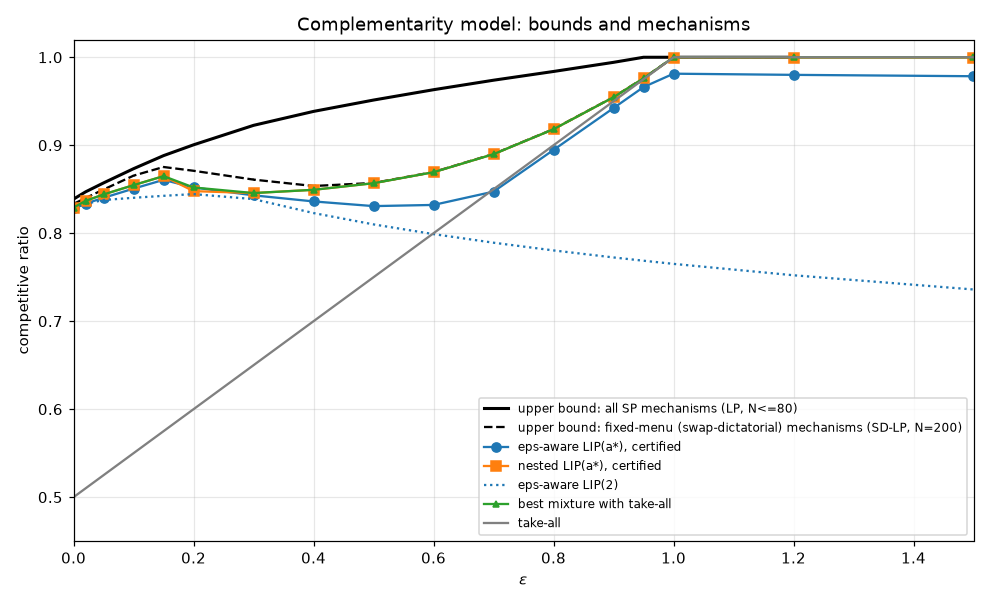
\includegraphics[width=0.95\linewidth]{figures/03_eps_overview.png}
\caption{Complementarity model: bounds and mechanisms as functions of $\varepsilon$. Black: LP
upper bound on all strategy-proof mechanisms ($N\le80$). Dashed: upper bound on fixed-menu
mechanisms (Theorem~\ref{thm:B}, computed by the menu LP at $N=200$). Blue/orange: certified
ratios of $\varepsilon$-aware and nested LIP with $a$ optimised per $\varepsilon$; dotted: $\varepsilon$-aware
LIP(2); green: best mixture of nested LIP with take-all; grey: take-all, $(1+\varepsilon)/2$.}
\label{fig:eps_overview}
\end{figure}

Figure~\ref{fig:eps_overview} summarises the section. Three things stand out. (i) The gap between
the dashed and the black curve - the \emph{price of dictatorship} - is about $0.1$ at
$\varepsilon=\tfrac12$ ($0.857$ vs $0.951$), far larger than in the additive model, where it is at most
$0.003$ (Theorem~\ref{thm:B} at $\varepsilon=0$). (ii) The worst case has moved: in the additive model identical types were the
easy case (ratio~1); with complementarities they become the hard one, since the first best pools
and a dictator splits. (iii) For $\varepsilon\ge1$ everything collapses to the trivial take-all. The
natural next question is whether a mechanism that reacts to agreement between the two reports
can close the gap; Section~\ref{sec:smd} gives one.
